% Chapter Template

\chapter{Introduction} % Main chapter title

\label{Chapter1} 

%----------------------------------------------------------------------------------------
%	SECTION 1
%----------------------------------------------------------------------------------------

\section{Original state}

\begin{figure}[h!]
	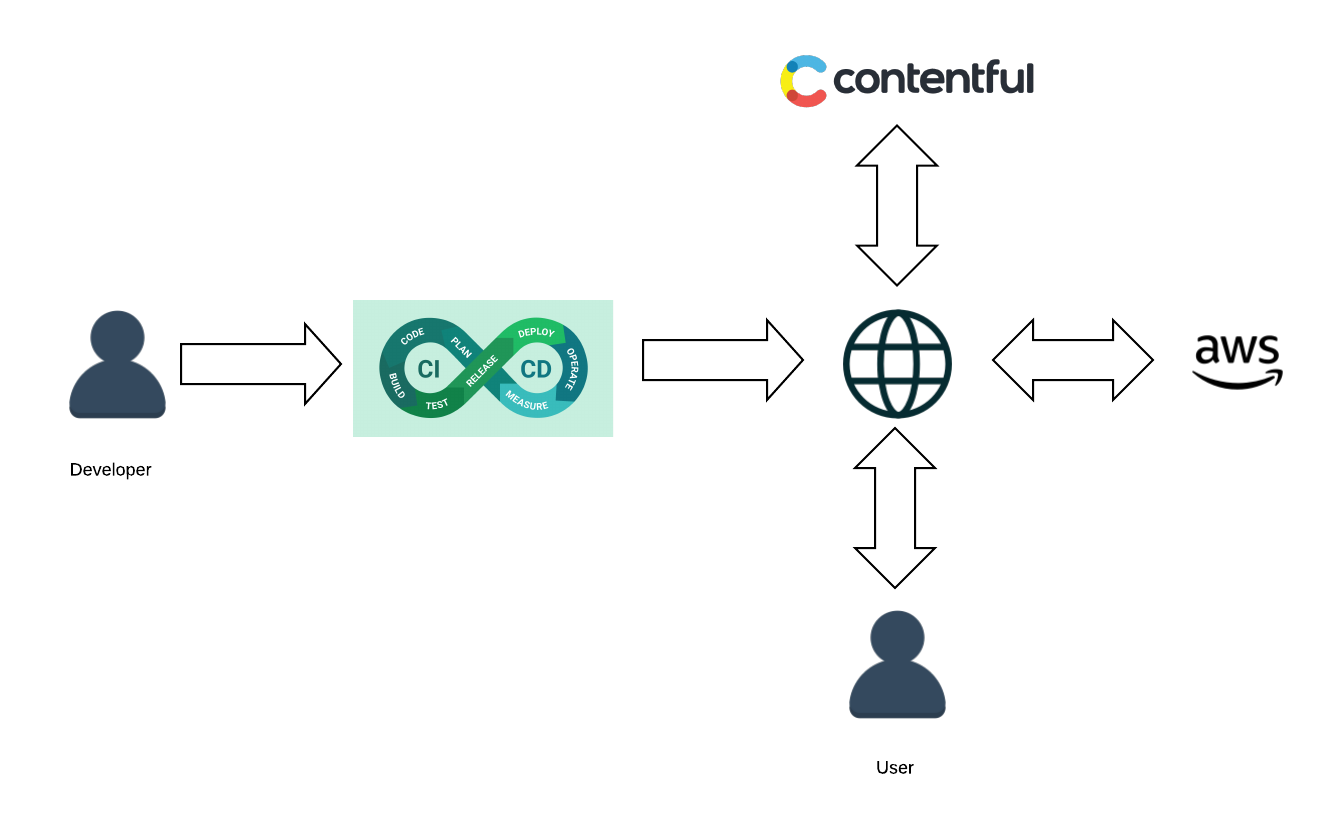
\includegraphics[scale=0.25]{original_flow}
	\caption{The original flow of the web application}
	\label{fig:original_flow}
\end{figure}


The inital state of the process we will investigate is a fairly typical web application. Developers write code which gets built and deployed by a CI/CD pipeline. The result are static files which are served by a webserver.

Users who visit the site receive these static files, after which the application will perform API requests to a CMS which returns the necessary assets. The application will also send API requests to a backend (hosted on AWS) for completing business logic.


\section{Stampix}

Stampix is a startup based in Belgium. It's main clients are businesses, businesses can purchase 'prints' with Stampix which they can then use for marketing/loyalty campaigns. 
The exact purpose always depends on the business, a concrete example would be "Sign up for our newsletter and receive 5 free photos!". So the business is responsible for distributing their purchased prints to the users.

Users who have received these prints can then visit the web application to select photos, crop/rotate/resize/... as needed and ultimately send their selection to Stampix servers. 
At this point, the responsibility of the web application ends and the backend processes take over. The photos are sent to printing partners for printing and distribution.

Stampix has many clients and since the primary use case is using the print for marketing purposes, the web application should be appropriately branded with the clients assets.
